
\documentclass[lnicst]{svmultln}
\usepackage{amssymb}
\setcounter{tocdepth}{3}

\usepackage{epsfig}
\usepackage{cite}
\usepackage{verbatim}
\usepackage{graphicx}
\usepackage{subfigure}
\usepackage[table]{xcolor}

\usepackage{url}
\urldef{\mailsa}\path|{collins, rajive}@cs.ucla.edu|
\usepackage[pdfpagelabels,hypertexnames=false,breaklinks=true,bookmarksopen=true,bookmarksopenlevel=2]{hyperref}

\begin{document}

\mainmatter  

\title{A Quantitative Comparison of Communication Paradigms for MANETs}

\titlerunning{A Quantitative Comparison of Communication Paradigms for MANETs}

\author{Justin Collins\and Rajive Bagrodia}
\authorrunning{A Quantitative Comparison of Communication Paradigms for MANETs}

\institute{University of California, Los Angeles\\
Los Angeles, CA\\
\mailsa }

\toctitle{A Quantitative Comparison of Communication Paradigms for MANETs}
\tocauthor{Justin Collins, Rajive Bagrodia}


\maketitle
\begin{abstract}
Mobile ad hoc networks (MANET) present a challenging area for application development. The combination of mobile nodes and wireless communication can create highly dynamic networks with frequent disconnections and unpredictable availability. Several language paradigms have been applied to MANETs, but there has been no quantitative comparison of alternative approaches. This paper presents the first quantitative evaluation of three common communication paradigms (publish/subscribe, RPC, and tuple spaces) compared within realistic MANET environments using real applications. We investigate the application-level performance of the paradigms and present a summary of their relative strengths and weaknesses. We also demonstrate the impact of wireless and mobility on application-level metrics, the most dramatic being delivery rates dropping to nearly 25\% and round trip times increasing up to 2000\% in a mobile scenario.

\end{abstract}

\section{Introduction}

%Mobile ad hoc networks (MANET) comprised of small, mobile, wireless devices present a new and challenging area for the development and deployment of applications. As consumer devices equipped with WiFi capabilities such as smartphones become more widespread, the possibility of impromptu networks also increases. While there has been a large amount of work focused on the networking stack, the application layer is not insulated from the challenges faced at the networking layers.

In mobile ad hoc networks (MANET), high nodal mobility causes frequent topology and route changes, making it difficult to maintain connections between nodes. Many routes in the network span multiple wireless hops which may experience dramatic and unexpected fluctuations in quality. The combination of mobility and wireless communication creates highly dynamic network topologies in which frequent, possibly permanent disconnections are commonplace. The dynamics of the network and the wireless channel requires changes to the networking stack and alternative solutions at the application level.

Middleware, frameworks, libraries, and languages have been proposed for meeting the challenges of developing mobile and ubiquitous applications. Quantitatively comparing these projects is difficult, since they are implemented in different languages, with different feature sets, and with varying levels of completeness. In this paper, we examine the fundamental differences in communication paradigms commonly used in projects, rather than the projects themselves. We accomplish this by evaluating representative implementations of each paradigm.

We also use real applications utilizing each of the paradigms, allowing us to investigate the impact of the paradigms on application-level metrics. Of prime importance to MANET applications is the performance of the communication model when the wireless channel and mobility are introduced. Therefore, we have evaluated the communication paradigms using a high-fidelity emulation of the network stack and detailed models of the wireless channel.

Since these communication models are common across multiple projects and are likely to be used in future projects, the results of this study have wide applicability. While previous work has qualitatively compared a subset of these paradigms or reported experimental results at the individual project level, we have investigated the performance characteristics of the underlying communication models themselves.

In this paper, we present the first quantitative comparison of three communication paradigms - publish/subscribe\cite{psfaces}, remote procedure calls\cite{rpc}, and tuple spaces\cite{linda} - using canonical implementations within real applications. Our results show wide variation in paradigm performance within the same scenario. Publish/subscribe provides fast, cheap message delivery, with a message overhead of 357 bytes and median round trip times of $<$400\textit{ms} even with mobility. RPC supplies good delivery ratios when a reply is expected, achieving a 94\% delivery ratio with mobility, while publish/subscribe and tuple spaces dropped to 75\% and 72\%. In the whiteboard application, however, tuple spaces were able to deliver all messages in 5 out of 6 scenarios, including a scenario in which RPC only delivered 25\%.

%The following sections present an overview of each paradigm, our evaluation architecture, and our quantitative results.

%\begin{table}
%\centering
%\caption{Communication Paradigms}
%\tiny
%\begin{tabular}{|c|c|c|} \hline
%\textbf{Paradigm} & \textbf{Temporally Uncoupled} & \textbf{Referentially Uncoupled} \\ \hline
%Publish/Subscribe & No & Yes \\ \hline
%RPC & No & Yes  \\ \hline
%Tuple Space & Yes & Yes \\ \hline
%\end{tabular}
%\label{fig:coupling}
%\end{table}

%\section{Communication Paradigms}\label{sec:paradigms}

%The three communication paradigms presented in this comparison are not unique to MANETs, but are based on traditional distributed and parallel computing concepts which are adapted to the MANET context.
%Since we wish to compare these models at the most fundamental level, we attempted to use canonical versions of each paradigm. The following sections describe how we have represented each model.

%It is useful to describe these communication paradigms in terms of temporal and referential coupling~\cite{distbook}. When a paradigm is temporally coupled, it requires the sender and the receiver to both be present when the message is sent. If it is temporally decoupled, a message will be stored and then delivered when the receiver becomes available. Referential coupling indicates whether or not the sender and receiver need to be directly aware of each other. A referentially coupled system explicitly addresses receivers, while a referentially uncoupled system does not need to know with which nodes it is communicating. 

%Both temporal and referential uncoupling are preferred in a MANET. If a paradigm is temporally uncoupled, it is more likely to be able to handle disconnections and changing network topologies. Referential uncoupling is useful, because it avoids the need for a centralized naming system and allows remote resources to be addressed using application-level semantics, rather than having to drop down to the network layer.

%\subsection{Publish/Subscribe}\label{sec:pubsub}

%Publish/subscribe is a messaging system in which nodes may subscribe to various topics. Nodes publish messages to certain topics, which are then delivered to their subscribers. Typically, there is a system of fixed nodes which serve as \textit{brokers} which manage subscriber lists and delivery of messages. In MANETs, the system must be completely distributed. Therefore, each node in our network can serve as a publisher, subscriber, and broker. However, the brokering system is completely transparent to the application layer. Published messages are not persistent, so only subscribers available when a message is published will receive it.

%Publish/subscribe is completely oriented towards group communication. The only method of communication is publishing a message to a topic. There may be zero or more subscribers to that topic, all of which will receive the message, provided the subscribers are available. One-to-one communication can only be achieved by coordination at the application layer. For example, two nodes may agree to communicate via a topic which they assume no one else will use.

%\subsection{RPC}

%Remote procedure call (RPC) is a form of message passing in which remote procedures or method invocations are syntactically similar or identical to local function calls, but the code is actually executed on a remote machine. When the procedure is called, arguments are copied to the remote machine, which executes the requested method and sends the resulting value back to the local machine.

%Like publish/subscribe, RPC is temporally coupled, since remote methods must be available at the time of the call. However, RPC is referentially uncoupled, since the application does not know which node it is communicating with, only that it supports a given method.

%Note that RPC inherently supports one-to-one two-way communication. Arguments to a method can be considered sending a message, and the return value of the method can be thought of as sending a reply message. RPC can also support group communication by invoking a given method on multiple remote hosts.

%\subsection{Tuple Spaces}

%Tuple spaces are a form of distributed shared memory. Conceptually, ordered tuples with typed fields are written out to a shared memory space. The tuples can then be read or retrieved by matching them to templates. Applications are associated with one or more tuple spaces, which allows them to access any tuples stored in that space. Three basic operations are defined to manipulate the tuple space which allow applications to take, write, and read tuples from the shared tuple space. Tuples are accessed by matching templates against existing tuples.
%\textit{in()} and \textit{rd()} use tuple templates which are matched against available tuples.
%There are also non-blocking versions of \textit{in()} and \textit{rd()} called \textit{inp()} and \textit{rdp()} which return immediately even when there are no matching tuples.

%Tuple spaces are both temporally and referentially uncoupled. Tuples may be read any time after they have been written to the tuple space, provided they have not been removed in the meantime. Where a tuple may reside is completely unknown to the application; all communication is performed by requesting a tuple matching a particular template. Tuple spaces easily support group communication, since a single tuple may be read by any number of nodes. One-to-one communication can be achieved by agreement on a particular tuple field, although this does not guarantee unintended receivers will not read or even remove the tuple.

%\begin{figure}
%\centering
%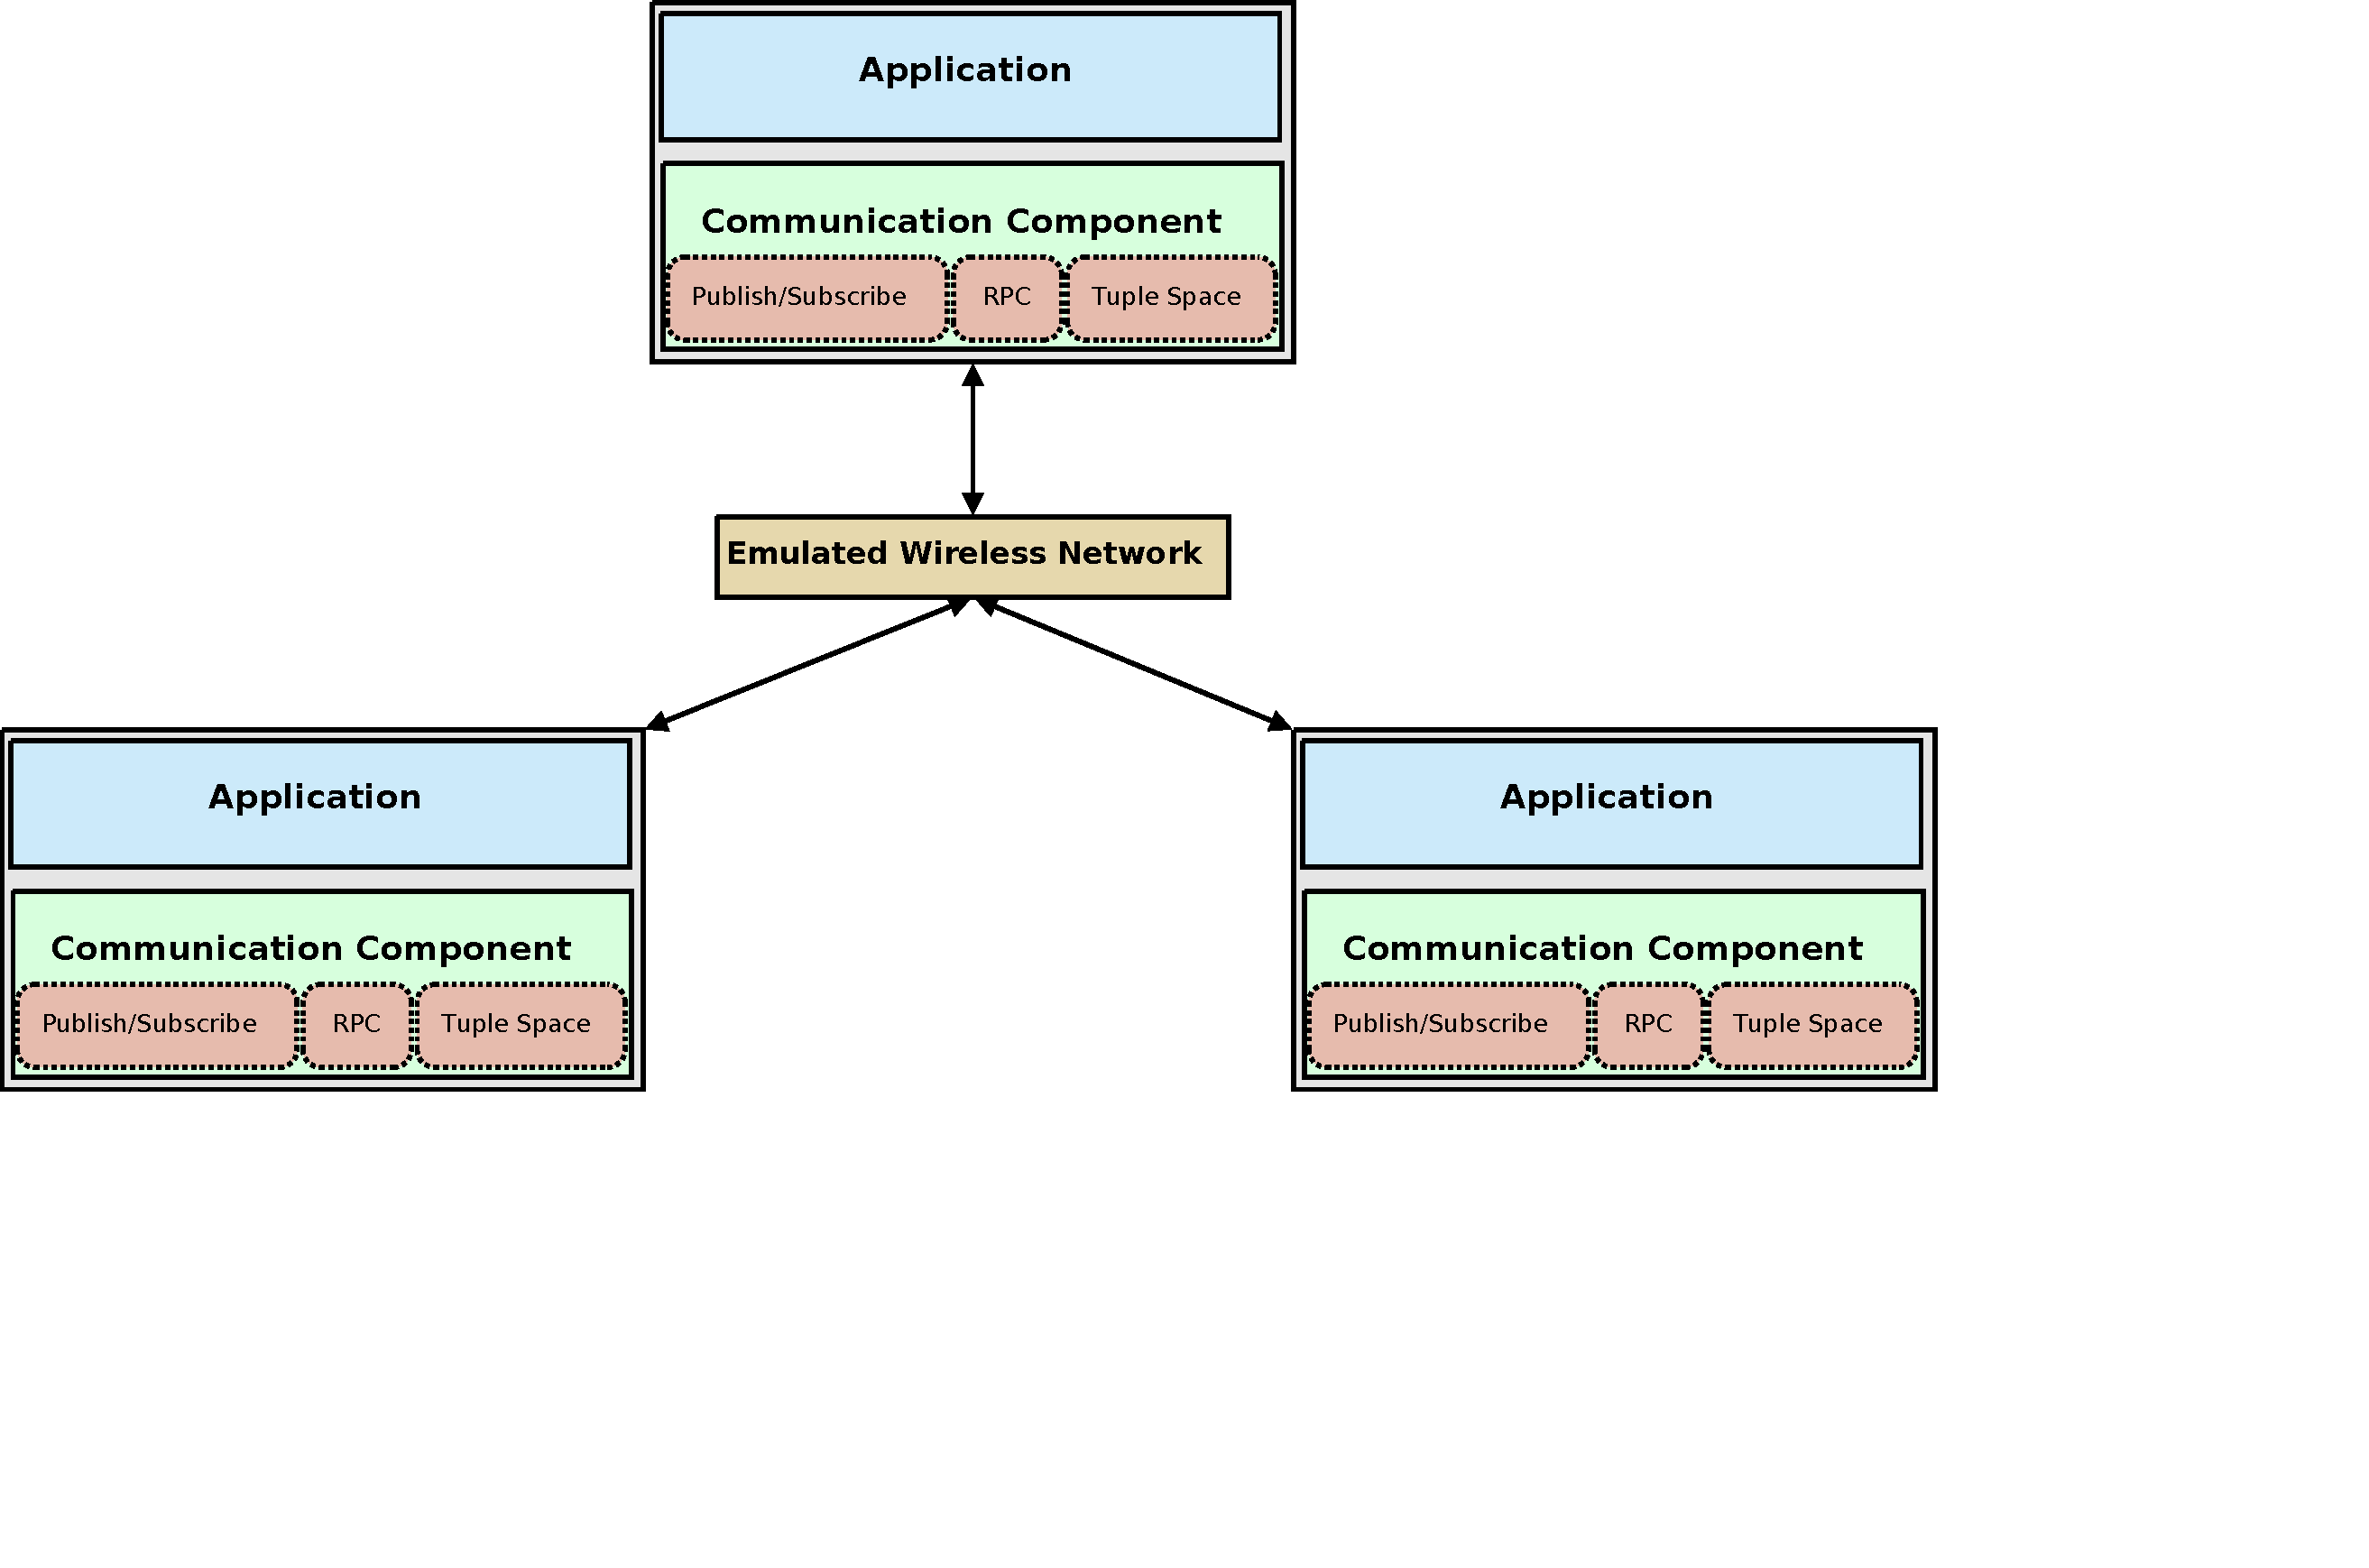
\includegraphics[scale = .26, clip, trim = 0px 190px 190px 0px]{figures/architecture.pdf}
%\caption{Evaluation Architecture}
%\label{fig:architecture}
%\end{figure}


\section{Evaluation Architecture}

The architecture used for this comparison has three layers: a network emulator, which provides a scalable and realistic MANET environment; the communication components, which implement the paradigms; and the applications which utilize the paradigms. The application is built on top of the communication component, which communicates over a regular wired network. The traffic from the network is routed through the network emulator, which provides a high fidelity simulation of the wireless network, intermediate nodes, and mobility. This allows applications to be written independently of whether the network is real or emulated.

\subsubsection{Network Emulation}

Because application-level performance is affected by variations in the wireless channel, mobility, and disconnection patterns, it is essential to have an accurate representation of the network stack and the wireless channel\cite{fidelity1,fidelity2}. EXata provides a high fidelity emulation of the entire network stack, using real MAC and routing protocols, as well as detailed simulation of the effects of the wireless channel and mobility, such as fading, shadowing, and path loss\cite{exata}. The emulator allowed us to run actual applications, rather than models, in a realistic representation of the MANET environment while retaining precise control of the variables in each experiment. This ensures our results are a fair comparison and not influenced by transient environmental effects.

%By using an emulator instead of a physical testbed, we are able to test each paradigm using exactly the same set of parameters, environmental factors, and mobility patterns.

\begin{figure}
\centering
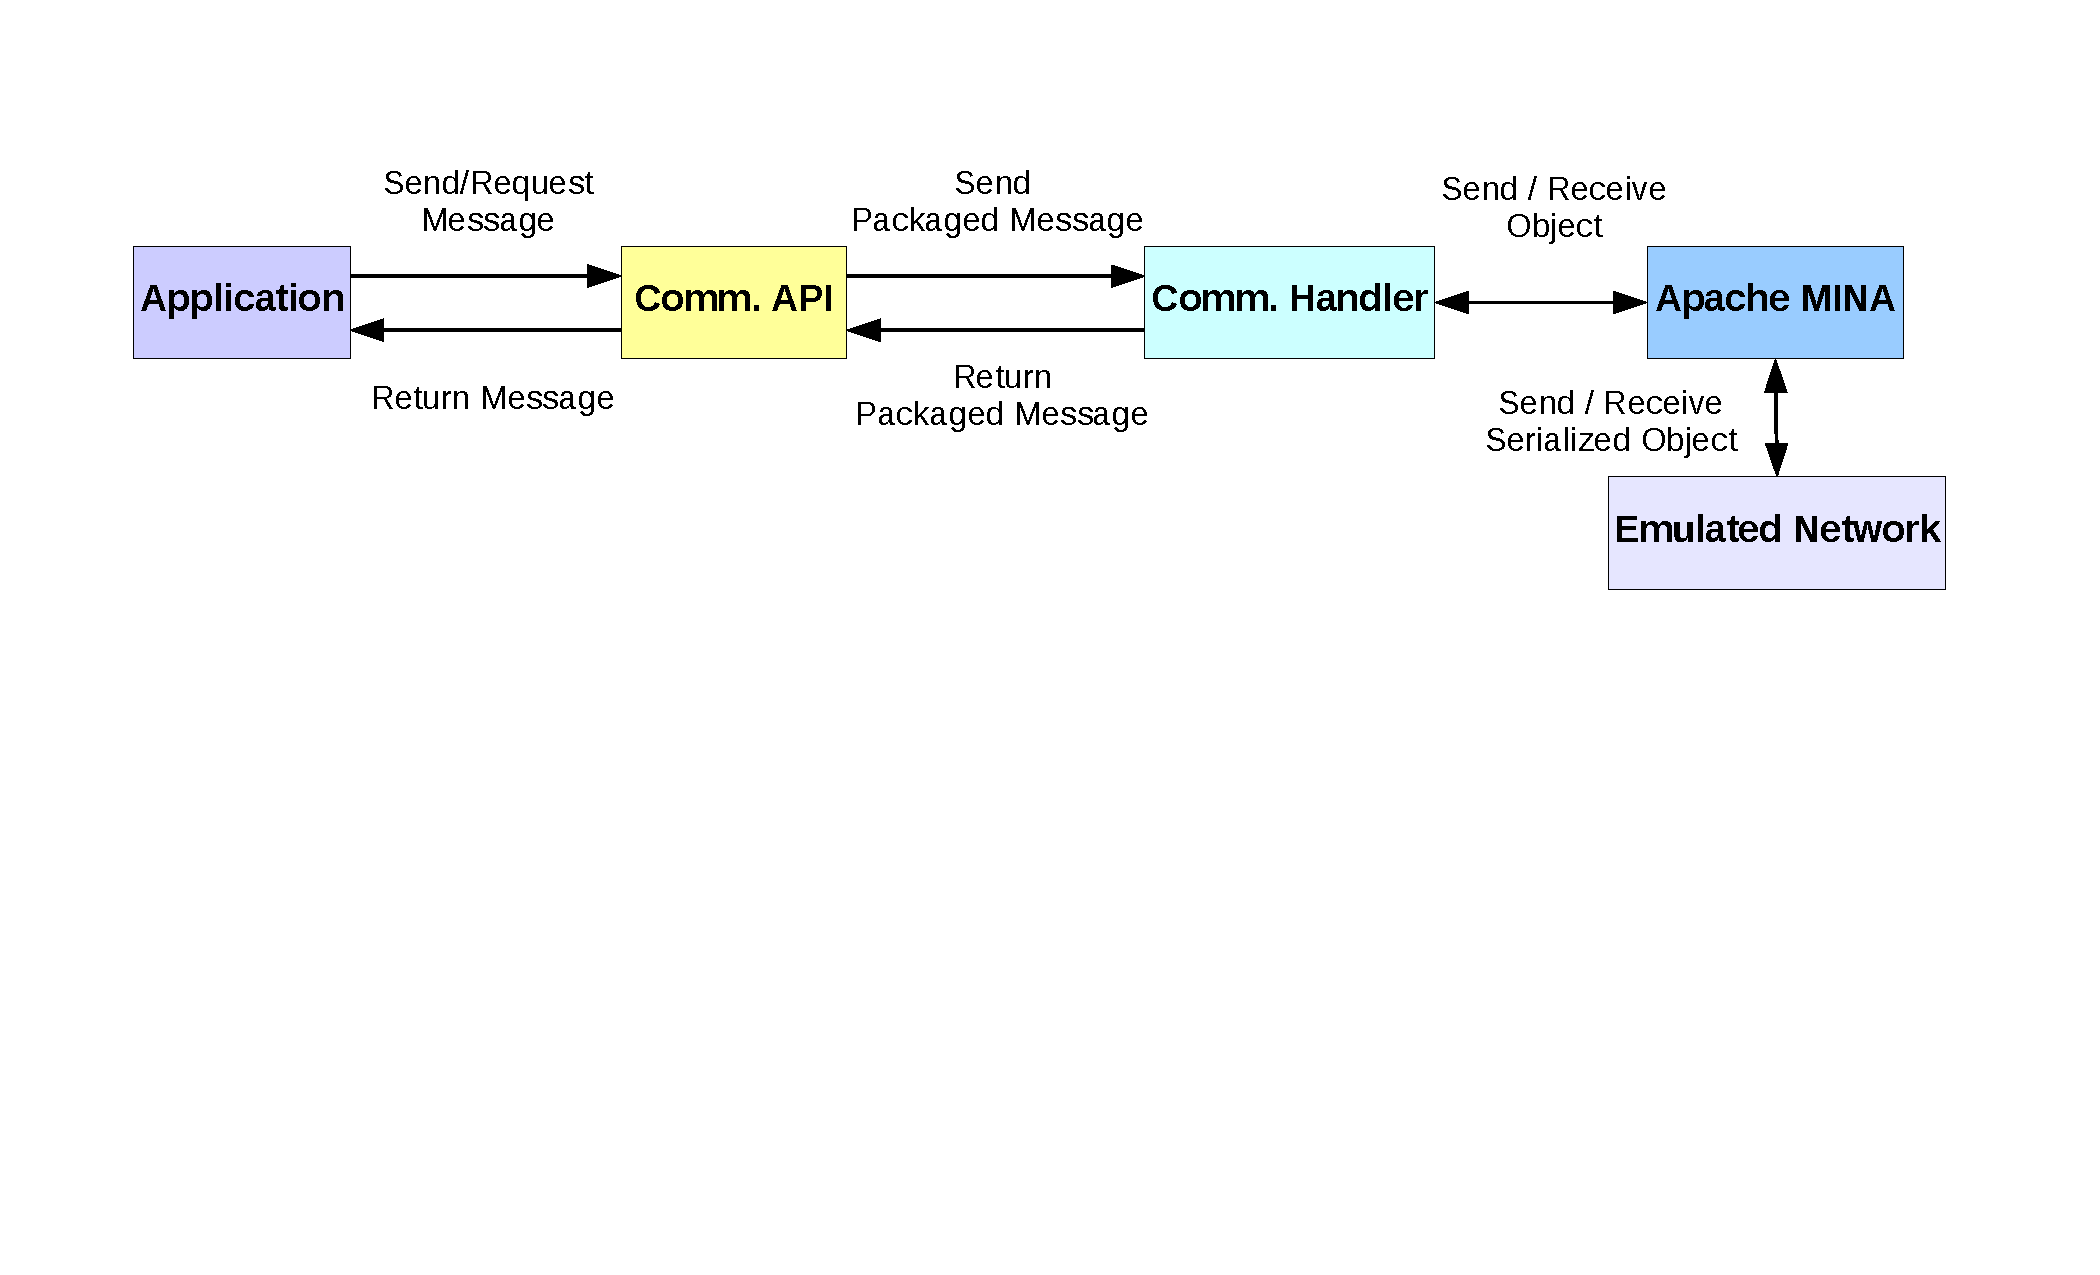
\includegraphics[width=\textwidth, clip, trim = 62px 325px 72px 80px]{figures/comm_comp.pdf}
\caption{Communication Components}
\label{fig:components}
\end{figure}

\subsubsection{Communication Components}

Each of the three communication paradigms are implemented in Java on top of Apache MINA\footnotemark, a high-performance networking library. A summary of the interaction between the application, the communication components, and the networking library is illustrated in Figure \ref{fig:components}. The libraries are intended to be functionally equivalent implementations of each paradigm to keep the comparison as fair as possible.

For publish/subscribe, we implemented a simple topic-based system. Publications to topics are broadcast to all subscribers available at time of publication. Our RPC implementation uses a reflection-based mechanism for invoking methods on remote objects, which are addressed by class. Parameters are copied to the remote machine and there is always a return value. The tuple space implementation we used is largely modeled on LIME~\cite{lime} and uses the same local tuple space library. All three implementations support unicast, multicast, synchronous, and asynchronous communication.

\footnotetext{Multipurpose Infrastructure for Network Applications: http://mina.apache.org/}

%This rest of this section describes how we implemented the canonical versions of the communication paradigms described in Section \ref{sec:paradigms}.

%\subsubsection{Publish/Subscribe}

%As stated in Section \ref{sec:pubsub}, it is not reasonable to expect any nodes to be reliable enough to serve as message brokers. Therefore, our publish/subscribe implementation assumes each node can serve as its own broker, which is not uncommon in MANET publish/subscribe systems\cite{psbrokers, psvsts}. Subscription requests are broadcast to all available nodes, which maintain lists of subscribers corresponding to a particular topic. For simplicity, topics are specified as simple strings in a flat address space. When an application publishes a message, it sends a copy of the message to all subscribers to the specified message topic. As is common in distributed publish/subscribe systems \cite{psfaces}, published messages are not persistent.

%\subsubsection{RPC}

%Our RPC implementation uses a simple reflection-based mechanism for invoking methods on remote objects. An application may enable remote availability for any Java object. Remote nodes can then search for an object by its class. When found, the application is given a handle to that object which the application can use to call a generic \textit{invoke()} method with the desired method name and parameters. The RPC library handles communication with the remote object and returns the resulting value from the method. This implementation avoids requiring any method stubs or compile-time knowledge of remote objects or method names.

%The library provides both synchronous and asynchronous remote invocations. Synchronous invocations will block until a remote object of the expected type is found and a return value is received. Asynchronous calls register a callback to handle the return value when it arrives.

%Our implementation also supports group communication. Group invocations attempt to invoke a given method on all known remote objects of the specified class. This must be done asynchronously, since multiple return values must be handled and it is not possible to know how many hosts will respond. The registered callback will be invoked each time a return value is received.

%\subsubsection{Tuple Space}

%Our tuple space implementation is largely modeled on LIME~\cite{lime} and uses the same local tuple space library called LighTS~\cite{lights}. This library provides storage of local tuples and matching of templates against the local tuple space. This allowed us to implement the communication features separately.

%While the tuples are logically located in a shared tuple space, they are actually stored locally. For example, an \textit{out()} operation does not actually involve any communication (unless there are existing requests for the output tuple). Operations on the tuple space, however, operate across the entire shared tuple space. When a \textit{rd()} or \textit{in()} is requested, a search is first performed on the local tuple space. If the request can not be completed locally, a request is sent to all known remote tuple spaces. The remote nodes then return a message indicating how many matching tuples they contain. The requesting node then chooses from the nodes with existing matches and requests the matching tuple itself.

%Requests which do not match any tuples are handled differently depending on whether the request is blocking or non-blocking. If a blocking request cannot be fulfilled, the request is stored and a reply will be sent if any future tuples match the request. A non-blocking request, on the other hand, will immediately return a message indicating zero matches.

%In our implementation, blocking requests will block the requesting application until the request can be filled. If no matching tuples exist at the time of the original request, the request will be periodically repeated until it is met. Non-blocking requests require a callback to be registered, which will be called when a matching tuple is received. 

%We also provide a \textit{reaction} mechanism\cite{lime}. An application may register a tuple template and a callback. The callback will be invoked when a matching tuple is added to the tuple space. This is equivalent to either periodically using a non-blocking request or making a blocking request in a separate thread, but is provided as a convenience.

%An application may also perform group requests. These are always asynchronous, due to the possibility of multiple matching tuples, but can still be considered blocking or non-blocking. A non-blocking group request will not be saved on remote nodes to be served later, while a blocking request will be.

\subsubsection{Applications}

The first application used for these experiments is a simple client-server application which can send messages between hosts. This provides a baseline for the performance results and allows us to easily test performance with varying message sizes and frequency. The second application is a shared whiteboard. Collaborative applications are often cited as use cases for MANETs and the shared whiteboard is a common example\cite{wb1, wb2, wb3, wb4}. This provides a non-trivial, realistic test case for each of the three communication paradigms.

%Each application has three functionally equivalent implementations, one for each of the communication paradigms.

\section{Experimental Results}

In the following sections, we present measurements of message delay and message delivery reliability for unicast and group communication, as well as for a non-trivial whiteboard application. We also examine the message overhead and the influence of routing algorithms. These experiments demonstrate the impact of the wireless network and mobility at the application level.

We compared application-level metrics using unicast and group communication in three network scenarios which are used throughout the experiments: a single hop, static network; a multi-hop, static network; and a fully mobile network. Each node in the emulated network is equipped with an 802.11b wireless interface. The two-ray model is used for path loss. Based on preliminary results, we used DSR\cite{dsr} as the routing protocol for the static scenarios and AODV\cite{aodv} for the mobile scenario.

%The implemented paradigms can be directly evaluated in several MANET scenarios using an emulator which provides high-fidelity representations of MANET environments. The repeatability of an emulator ensures that each paradigm can be evaluated in exactly the same situations and scenarios.
%Rather than comparing the utility and performance of the paradigms theoretically, the emulation approach allows them to be evaluated within actual applications. This more closely reflects their eventual purpose: the development of applications which will execute on a MANET.

The mobile scenario uses random waypoint mobility with a pause time of 30\textit{s} and maximum speed of 1 meter/second, representing pedestrians carrying handheld devices. The nodes move within a 1500\textit{m} x 1500\textit{m} indoor space where transmission range is limited to 50m. To avoid network segmentation, the scenario ensures there are always possible routes between any two nodes by having four fixed nodes. The mobility pattern in each experiment is identical.

%The emulation environment is provided by EXata\cite{exata}, a network emulator which allows actual applications to run on an emulated wireless network in real time. EXata provides a high fidelity emulation of the entire network stack and detailed simulation of the wireless channel. This provides the realistic environment required for accurate assessment of the paradigms while also facilitating repeatability and fairness\cite{fidelity1,fidelity2}.

%However, the remainder of the nodes are highly mobile and routes between nodes change frequently. 
%In the group communication experiments, Node 1 is the sender.



\subsection{Unicast Communication}

\subsubsection{Message Overhead}

\begin{table}
\centering
\caption{Message Sequence Overview}
\small
\begin{tabular}{|c|c|c|c|c|} \hline
Paradigm & Sender & Receiver & Size (bytes) & Overhead (bytes) \\ \hline
\rowcolor[gray]{.80}
Publish/Subscribe & & & & \\ \hline
& & Subscribe & 175 & \\
\rowcolor[gray]{.80}
& Publish & & 1182  & \\ \hline
& & \textit{Total} & 1357 & 357  \\ \hline
\rowcolor[gray]{.80}
RPC & & &  & \\ \hline
& Search & & 146 &  \\ 
\rowcolor[gray]{.80}
& & Search Reply & 187 &  \\
& Invoke & & 1238 & \\ 
\rowcolor[gray]{.80}
& & Return Value & 152 &  \\ \hline
& & \textit{Total} & 1571 & 571  \\ \hline
\rowcolor[gray]{.80}
Tuple Space & & &  & \\ \hline
& & Search & 608  & \\ 
\rowcolor[gray]{.80}
& Search Reply & & 133  & \\ 
& & Tuple Request & 588 &  \\ 
\rowcolor[gray]{.80}
& Tuple Reply & & 1586  & \\ \hline
& & \textit{Total} & 2915 & 1915  \\ \hline
\end{tabular}
\label{fig:messages}
\end{table}

\paragraph{Application Overhead}\label{sec:app_overhead}

The first step of our experimental evaluation of these three paradigms is discovering the basic cost of communication. Table~\ref{fig:messages} provides an overview of the sequence of messages involved when using each of the communication paradigms in the simple case of a single sender and a single receiver sending a 1KB payload. The total size includes the 1KB payload.
%The message sizes in Table~\ref{fig:messages} indicate the number of bytes sent from the application to the network layer.
Publish/subscribe requires only two messages to be sent: one to subscribe to a topic and one to publish. Since publish/subscribe only needs to add a string indicating a topic, there is very little overhead added to the original message.

RPC first sends out a query to find the desired remote object. Once found, it sends a second message to invoke the method and transfer any arguments. The final message in the sequence is the return value from the method, which is dependent on the size of the return value.

%In Table we present the simplest case, which is returning a null value.

Tuple spaces require the same number of messages as RPC, but the overhead is 2.3 times higher. Except for the search reply messages, all messages include a tuple object, making them larger than the simple messages exchanged in RPC.


\begin{figure}
\centering
\mbox {
\subfigure[Bytes per Message] {\label{fig:overhead-bytes}
	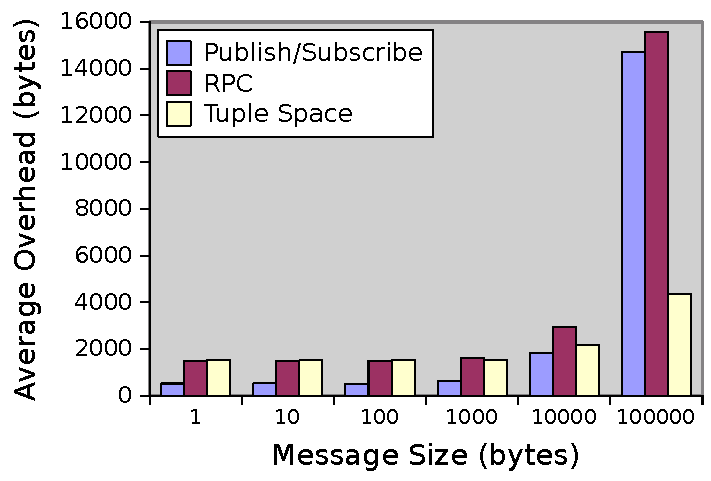
\includegraphics[width = .48\textwidth]{figures/message-overhead-bytes.pdf}
	}
\subfigure[TCP Packets per Message] {\label{fig:overhead-packets}
	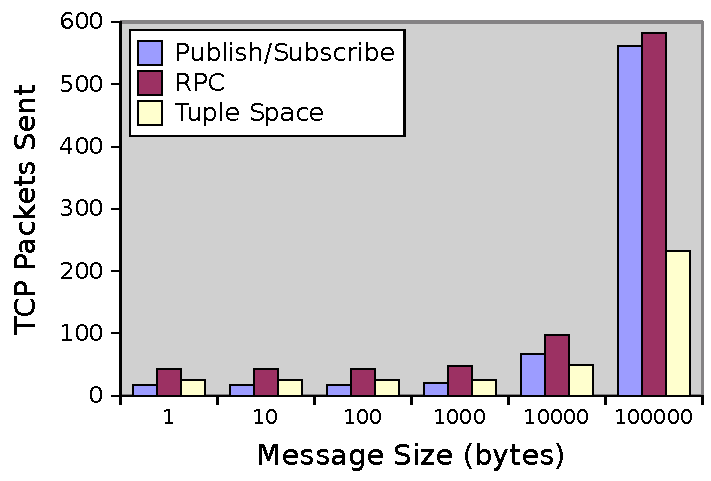
\includegraphics[width = .48\textwidth]{figures/message-overhead-packets.pdf}
	}
}
\caption{Average Message Overhead}
\end{figure}


\paragraph{Network Overhead}

While Table~\ref{fig:messages} indicated the overhead added at the application layer, Figure~\ref{fig:overhead-bytes} shows the average amount of TCP traffic which is sent over the network for a single message, calculated as \textit{bytes sent} - \textit{message size}. These results use the single hop static scenario and are averaged from 50 messages.

The results are fairly constant until the packet size is exceeded. There is some increase at 10KB, and a dramatic increase at 100KB. Figure~\ref{fig:overhead-packets} shows the same data in terms of TCP packets and indicates the cause of the sharp increase in traffic at 100KB is the result of packet fragmentation.

Despite having large message sizes, tuple spaces have much lower overhead in terms of TCP traffic. This difference arises from a side issue related to TCP send window sizes. For tuple spaces, where the receiver initiates the connection, the TCP send window size grows to accommodate larger packet sizes. With RPC and publish/subscribe, the send window size remains constant, causing the large messages to be split into many more packets. 
%For RPC and publish/subscribe, the sender initiates the TCP session, while in tuple spaces it is the receiver (of the tuple) which initiates the TCP session.

\subsubsection{Message Reliability}

How reliably a communication paradigm handles message delivery has a direct impact on the application layer. The more reliable the communication paradigm, the less responsible the application is for handling lost messages. We measured reliability in terms of message delivery. In the single hop scenario, all paradigms achieved 100\% delivery and figures~\ref{fig:mgdel} and \ref{fig:mgdel} indicate nearly perfect message delivery for all the paradigms in the unicast scenario. Publish/subscribe performed the worst and still only lost 4 messages.
%However, this is not unexpected, since publish/subscribe sends out publications immediately, whether or not any subscribers are present.

\subsubsection{Message Delay}

Message delay is another important application-level metric, as it determines how quickly information is transferred and the freshness of the application's information. Figures \ref{fig:shgps}, \ref{fig:shgrpc}, and \ref{fig:shgts} show delay in terms of round trip times for each paradigm in a single hop scenario. The majority of the messages in each paradigm are under the 200\textit{ms} mark, with just a few wayward messages taking longer. Even for tuple spaces, 80\% of the messages take less than 400\textit{ms} to complete their round trip. However, some messages take much longer, up to 8\textit{s}. For tuple spaces, this is partially due to the complexity and overhead of the messages required to perform the round trip message delivery.

However, the time delay for tuple spaces in the single hop scenario is also related to the pull (rather than push) nature of the paradigm. A tuple is time-stamped when it is output, but the tuple is not actually sent to the receiver until the receiver requests it. The same situation happens on the return trip, when the tuple must be pulled back to the original sender. Any delays in this process cause the round trip time to increase.

On the other hand, publish/subscribe messages are sent out almost immediately after being timestamped. Nearly all the delay is caused by the network itself. RPC has more potential for delays since it must find the remote method before invoking it. However, the return message can reuse the existing TCP connection, which appears to provide an advantage over tuple spaces.

%The multi-hop scenario introduces more message latency, as seen in Figures \ref{fig:mhgps}, \ref{fig:mhgrpc}, and \ref{fig:mhgts}. Again, most messages complete the round trip very quickly ($<$300\textit{ms}), but the maximum times for publish/subscribe and RPC increased from 383\textit{ms} and 110\textit{ms} to 1537\textit{ms} and 902\textit{ms}, respectively. Not only does it take longer due to the packets needing to traverse multiple hops, there is also delay introduced by the time to find routes. In the single hop scenario, routes are set up at the beginning of the scenario and there is virtually zero routing activity after that. On the other hand, the multi-hop scenario performs routing updates throughout the run time of the scenario.

The mobile scenario introduces even greater delays. Routes are changing frequently and may be several hops long. While the publish/subscribe and RPC results are clustered around 100\textit{ms} and remain under 500\textit{ms}, the tuple space values are considerably higher with a median at 256\textit{ms} and a high of nearly 20\textit{s}. This is again due to the pull nature of tuple spaces and the overhead seen in Section \ref{sec:app_overhead}.

\subsection{Group Communication}

Group or multicast communication is a useful but more complex part of MANETs, where information and resources are often disseminated in a peer-to-peer manner. Group communication differs significantly from unicast communication. Given the mobile characteristics and decentralized nature of MANETs, a group's membership may be in constant flux, so it is unlikely a sender has perfect knowledge of the members of the group. The time difference between replies from members of the group may vary greatly, and the initiating node cannot know how many replies to expect.
%Consider an application which makes a request for some information from all nearby nodes. It is difficult to know how long it should wait to receive all replies, because it is not known how many replies should be expected, yet it is entirely possible that an application will receive multiple replies from the group. It is also possible to have a large time difference between replies from different nodes.

We have investigated how well each paradigm handled group communication by again evaluating message delay and message delivery reliability, but with multiple receivers.

%\subsubsection{Round Trip Application}\label{sec:rtapp}

%The method for achieving group communication is slightly different for each paradigm. In publish/subscribe, there are two topics: one for outgoing messages and one for incoming messages. The sending node publishes a message containing a timestamp to the outgoing topic. When an outgoing message is received, the receiving node republishes the message to the incoming topic. The round trip time is then calculated when the sending node receives the incoming copy of the original message.

%In RPC, a group method call is asynchronously invoked with a timestamp as the parameter. A group invocation will attempt to invoke all available copies of the remote method and register a callback to handle the return values. In this case, that callback will receive the original timestamp and calculate the round trip time from it.

%Since tuple spaces only support pull operations, the situation is inverted. Receivers request an outgoing tuple, which will contain a timestamp. The sender outputs a proper tuple with a timestamp, which is then sent to the requesting receivers. The sender then requests a reply tuple and registers a callback to handle the tuple when it arrives. Upon receiving the tuple with a timestamp, the receiver will output a reply tuple containing the same timestamp. This tuple will be sent back to the original sender, which can then compute the round trip time. This is illustrated in Figure \ref{fig:tuple-failure}.

\begin{figure}
\centering
\mbox {
%\subfigure[Single Hop Scenario] {\label{fig:sgdel}
%	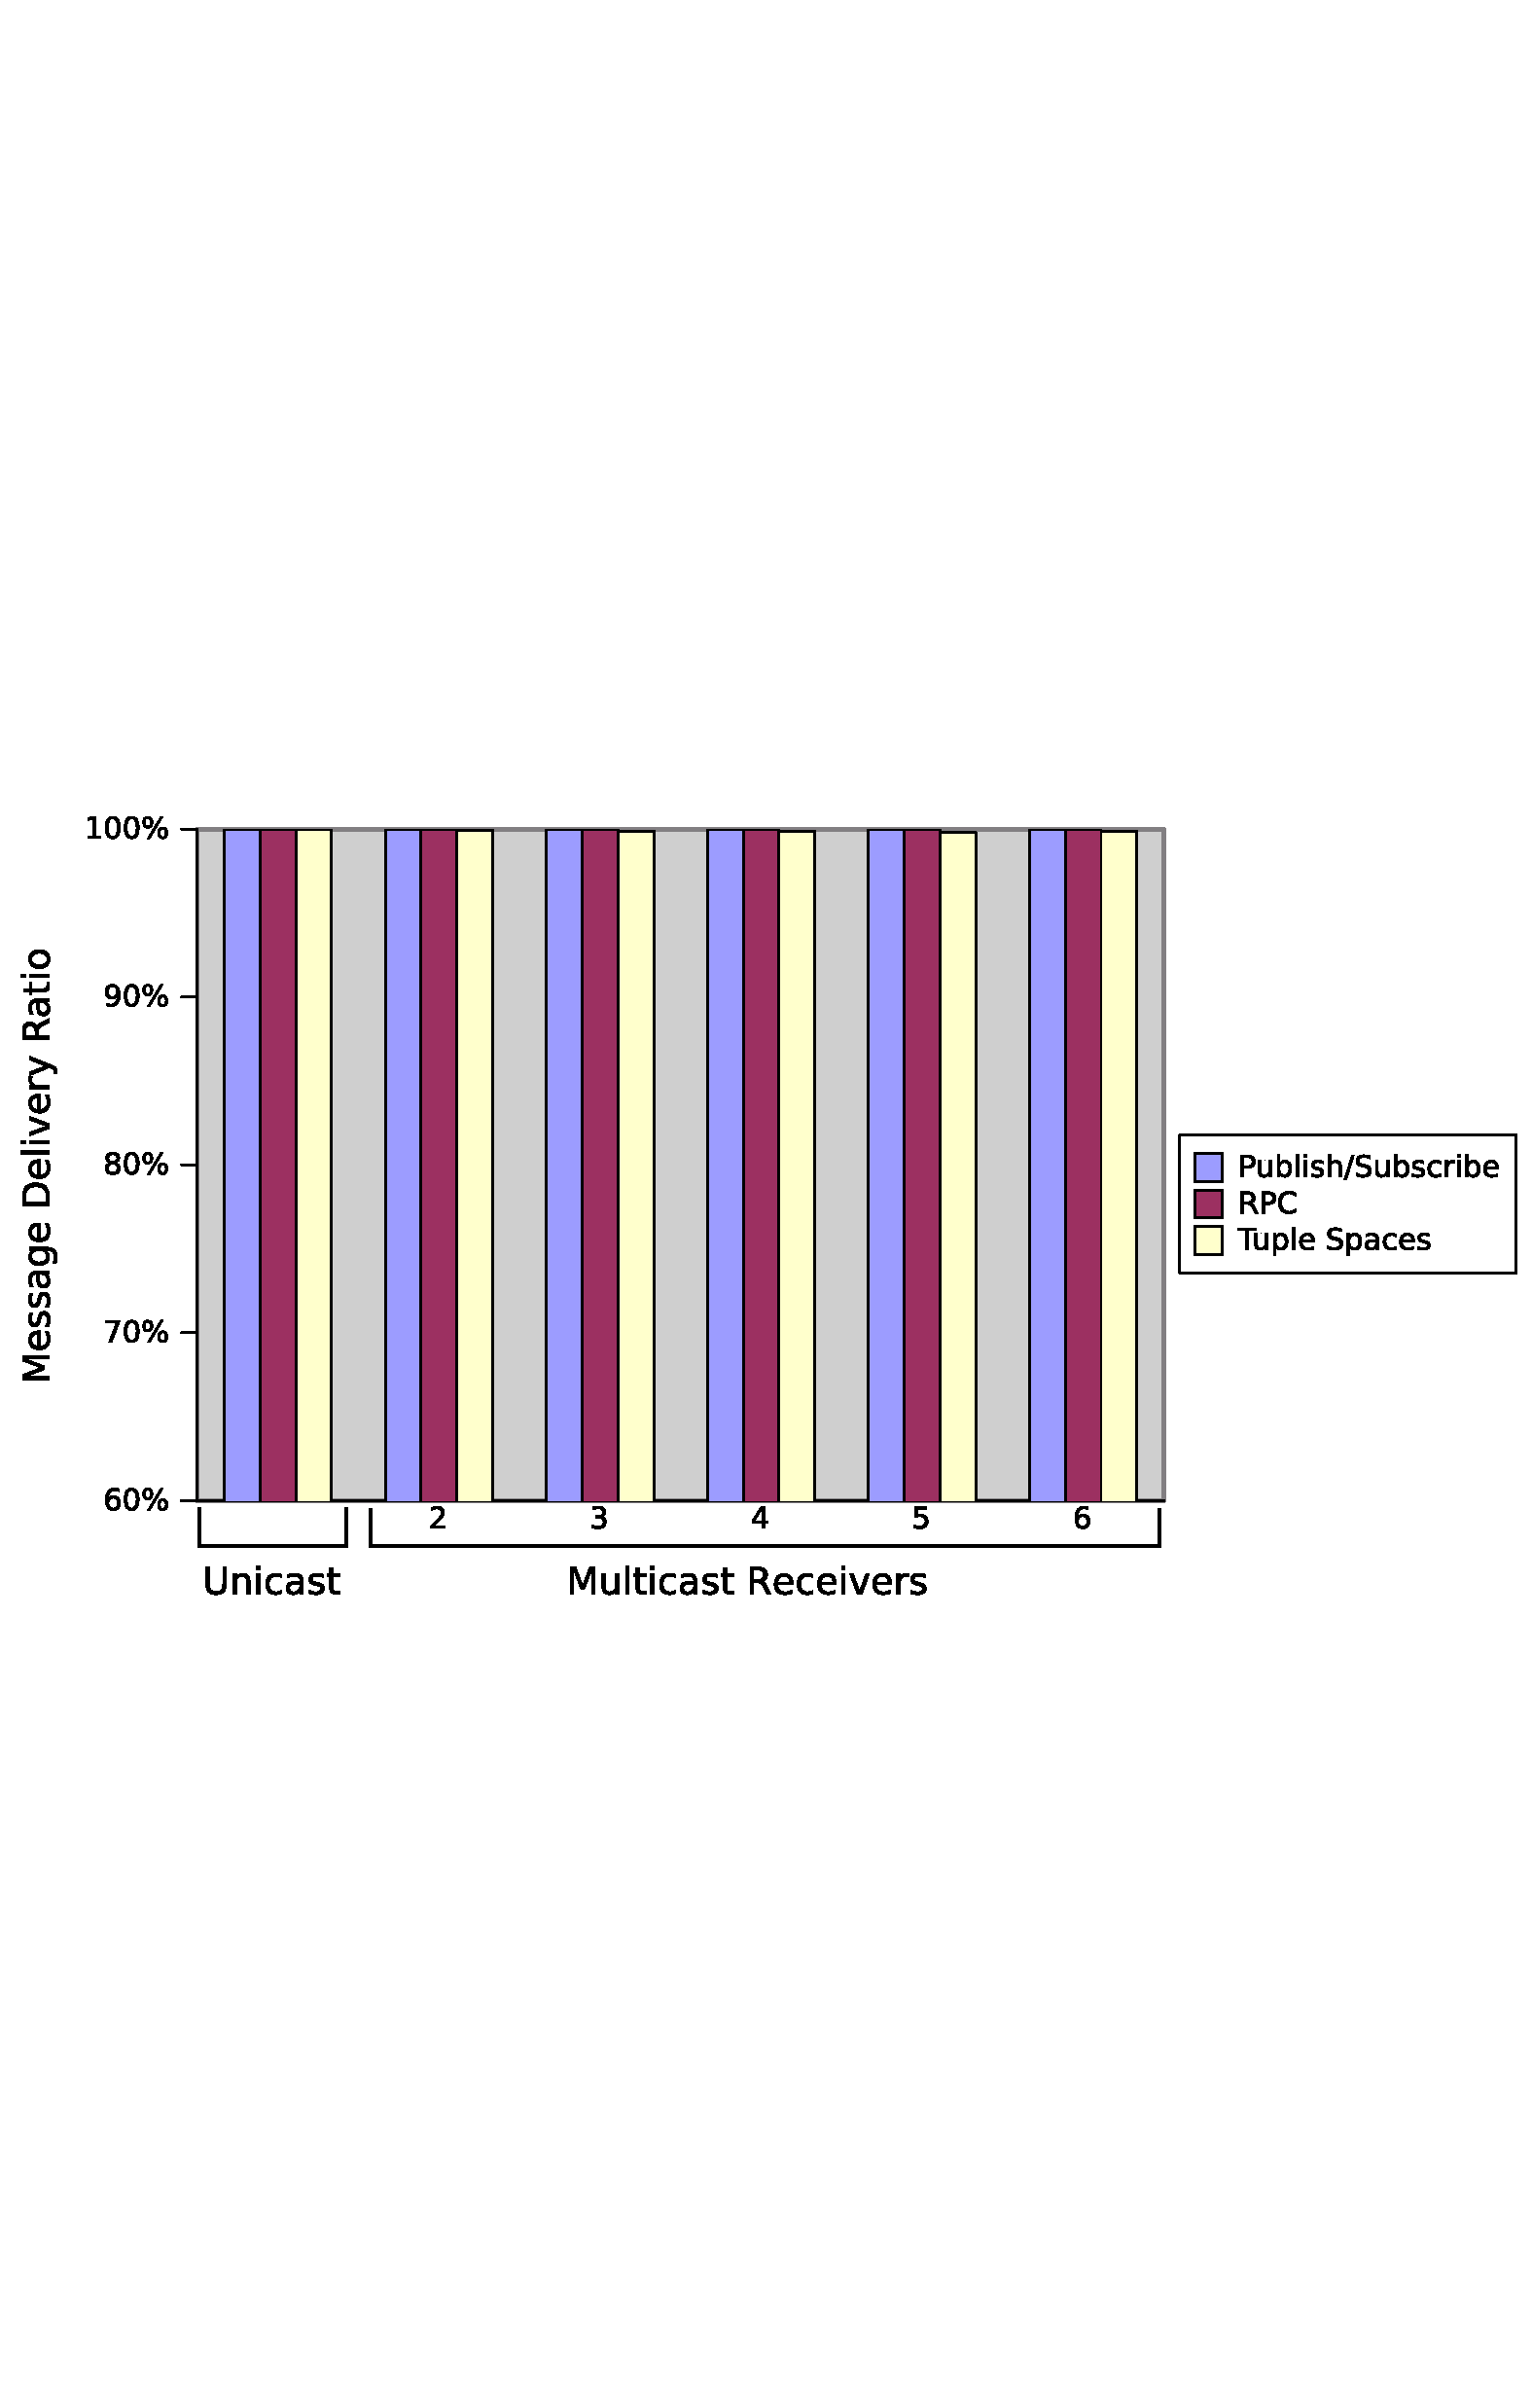
\includegraphics[width = 0.49\textwidth, clip, trim = 0px 400px 0px 400px]{figures/single-hop-group-delivery.pdf}
%	}
\subfigure[Multihop Scenario] {\label{fig:mhgdel}
	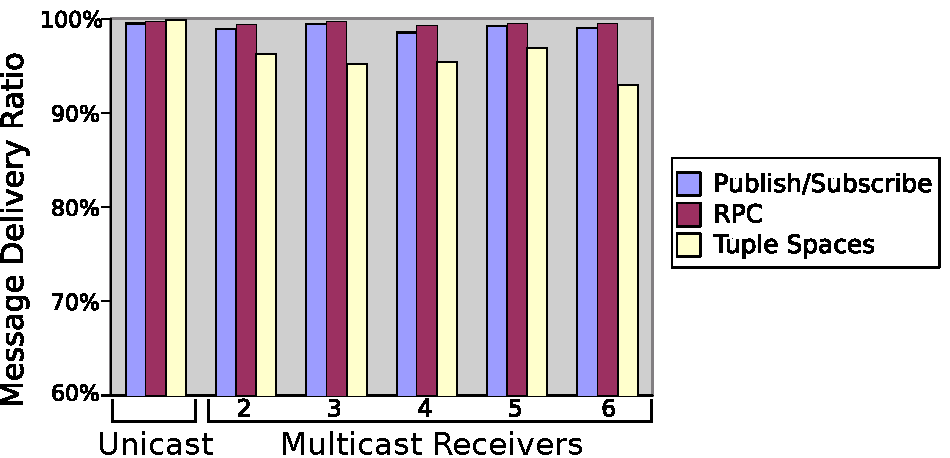
\includegraphics[width = 0.59\textwidth, clip, trim = 0px 0px 0px 0px]{figures/multi-hop-group-delivery.pdf}
	}
	
\subfigure[Mobile Scenario]{\label{fig:mgdel}
	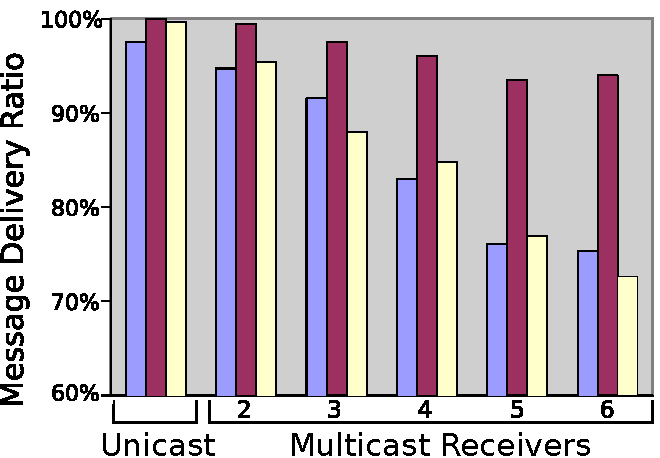
\includegraphics[width = 0.40\textwidth, clip, trim = 0px 0px 0px 0px]{figures/mobile-group-delivery.pdf}
	}
}
\caption{Message Reliability}
\end{figure}


\subsubsection{Message Reliability}\label{sec:group_reliability}

With this application, message reliability refers to messages which make the circuit from the sender to the receiver and back to the sender. This is useful, for example, in situations where a sink node aggregates information from other nodes.

Figures \ref{fig:mhgdel} and \ref{fig:mgdel} show the percentage of messages successfully completing the round trip. The single hop scenario is not shown, as all paradigms achieved $>$ 99\% reliability in that scenario. In the multi-hop scenario, there are more losses even without mobility, but there is no significant trend as the number of receivers increases.

RPC has a slight advantage with this metric, as it will wait until at least one receiver is available. Publish/subscribe and tuple space will send out messages whether or not any receivers are available at the time. However, none of the communication paradigms will retry a message which is lost in transit. A message lost anywhere in the circuit causes the entire attempt to be reported as a failure.
%For example, if RPC is able to connect to a remote method and invoke it, but never receives a return message, it will not attempt to invoke the method again. Since these results require a message to complete the round trip circuit, there are multiple opportunities for message delivery to fail. 

This contributes to tuple spaces showing the lowest delivery ratio (93\%) in the multi-hop scenario and a low delivery ratio (72.6\%) in the mobile scenario. While tuple spaces can easily handle the delivery of the outgoing tuple, it is more difficult to guarantee the return of the reply tuple. If a node is not available to receive the request broadcast for a reply tuple, then the reply will never be sent even if the original outgoing tuple is received.
%Figure \ref{fig:tuple-failure} illustrates why this is the case. The interaction in the ideal scenario assumes the sender and receiver are present for the entire interaction. In the second scenario, however, the receiver moves away from the sender after sending the initial request for an outgoing tuple. In step 3, the sender sends the reply request, but it cannot be delivered. When the receiver returns, it repeats its request for an outgoing tuple, because it is a blocking request which has not yet been satisfied. The sender satisfies the request, but the reply is never sent since the receiver never receives the reply request.

%\begin{figure}
%\centering
%\mbox {
%	\subfigure[Ideal Scenario] {
%		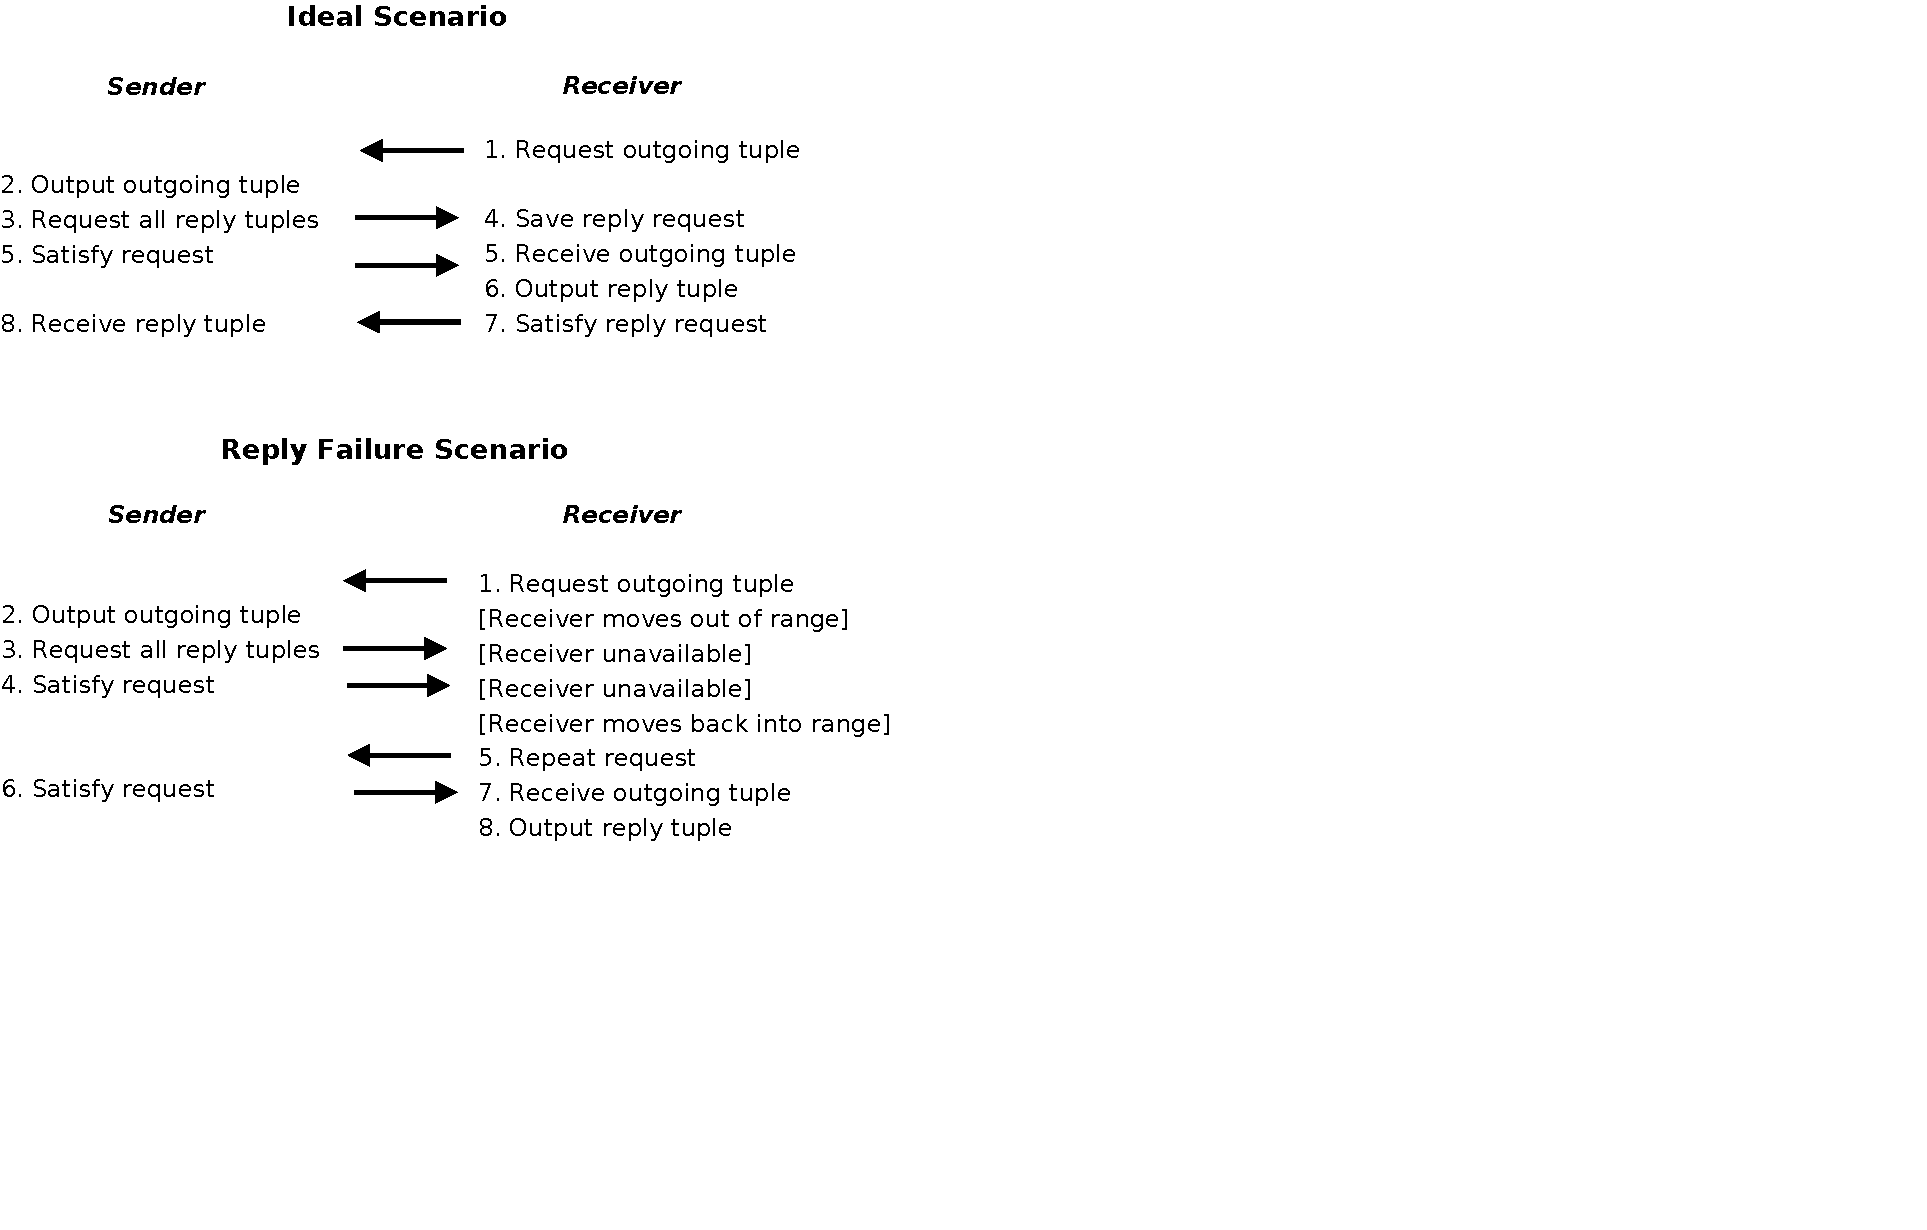
\includegraphics[scale = .40 , clip, trim = 0px 400px 500px 35px]{figures/tuple-failure.pdf}
%	}
%	
%	\subfigure[Failure Scenario] {
%		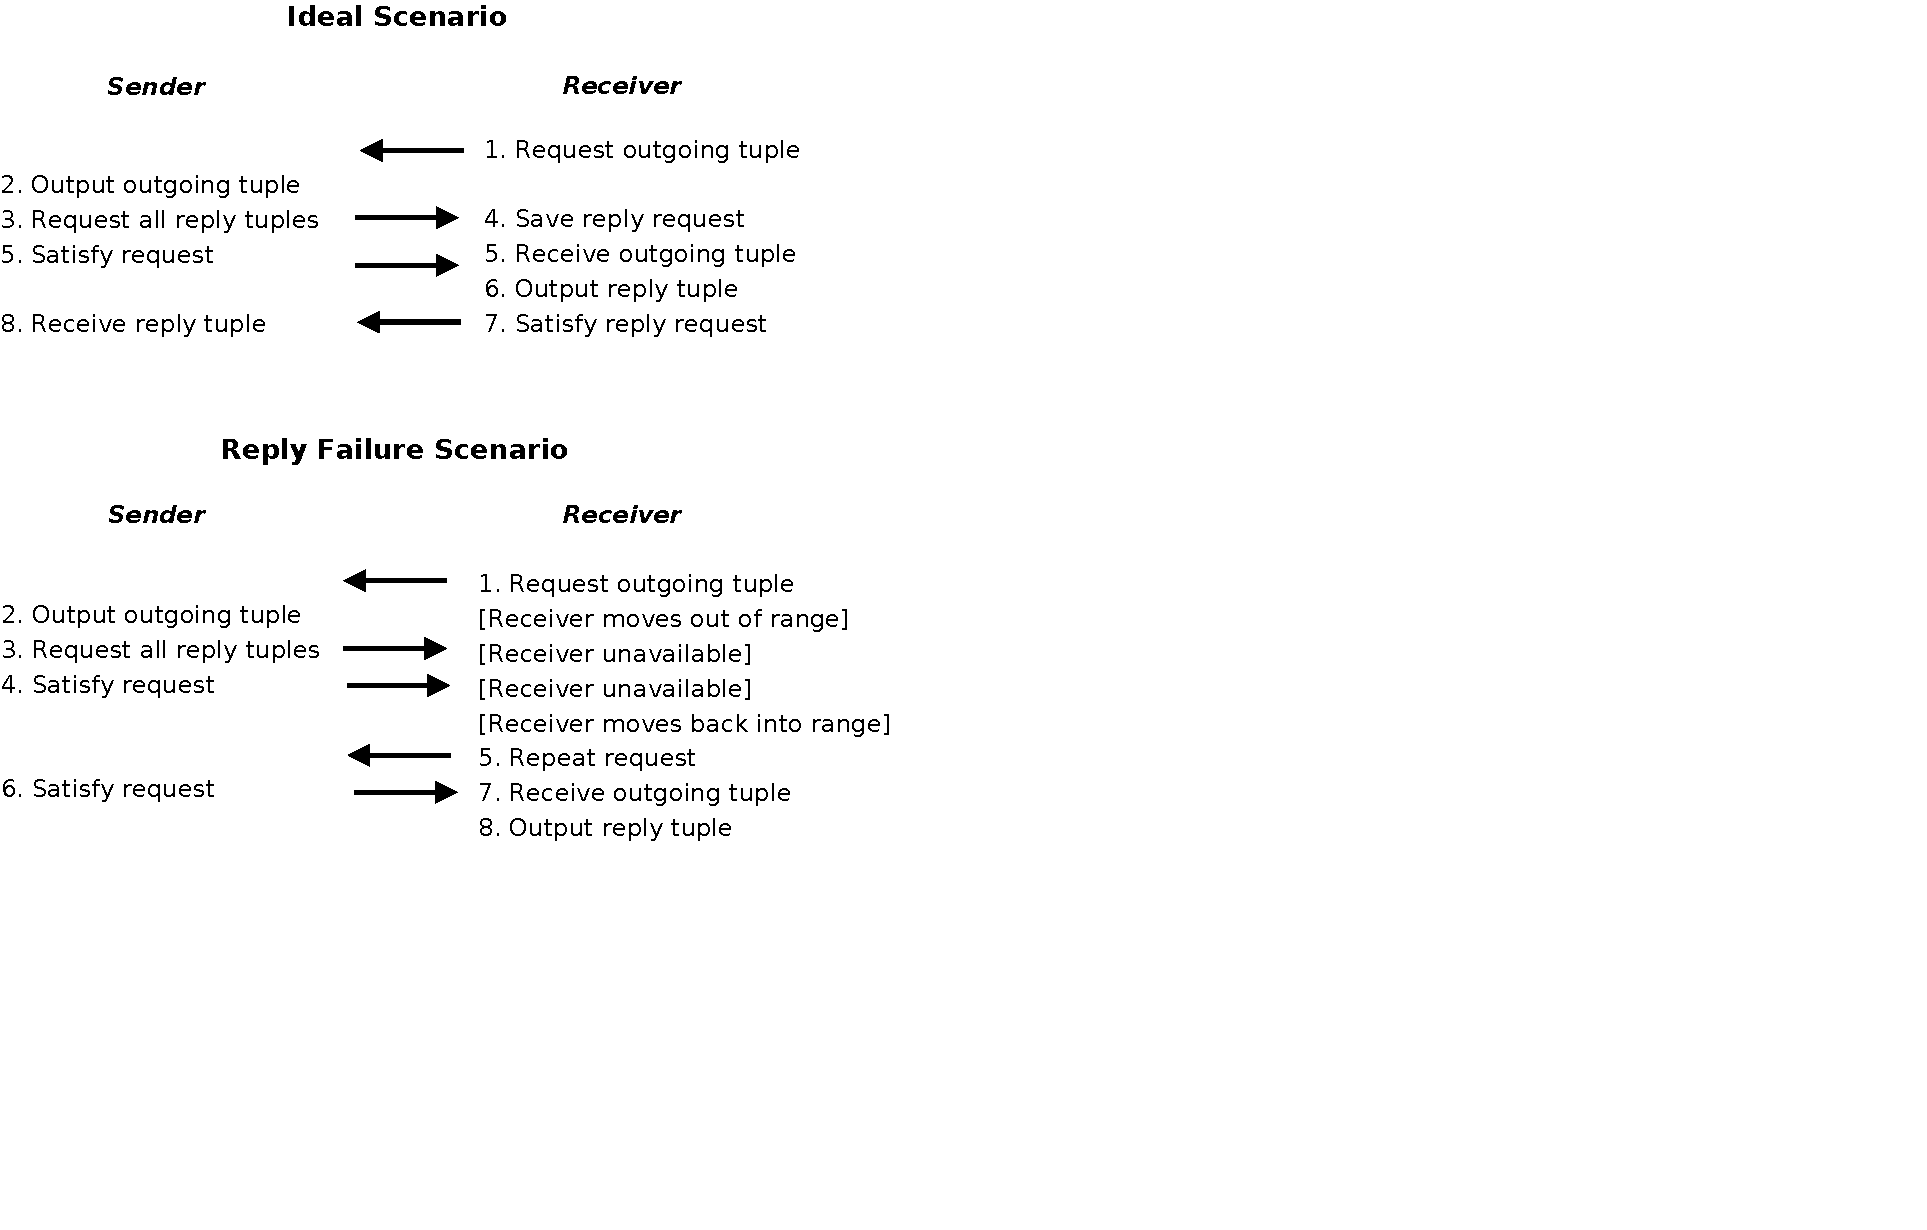
\includegraphics[scale = .40 , clip, trim = 0px 180px 450px 230px]{figures/tuple-failure.pdf}
%	}
%}
%\caption{Tuple Space Round Trip Application}
%\label{fig:tuple-failure}
%\end{figure}

%The solution to this situation would be to repeat the request for the reply tuples. However, the reply request is a group request. Retries are problematic for group requests, because it is unclear when a group request has been completely satisfied. While a normal \textit{rd()} \textit{or in()} operation is satisfied by a single tuple, there is no upper bound on how many tuples may be available to satisfy a group request, so the requester cannot know when to cease retrying. The LIME\cite{lime} project defines a group request as non-blocking and only operating on the current state of the tuple space. This solution would fail in \textit{both} exchanges shown in Figure \ref{fig:tuple-failure}, as the reply request may be received before the original request is satisfied. Therefore, we compromised by using blocking group requests, but without retries.

\begin{figure}
\centering
\mbox {
	\subfigure[Publish/Subscribe - Single Hop] {\label{fig:shgps}
	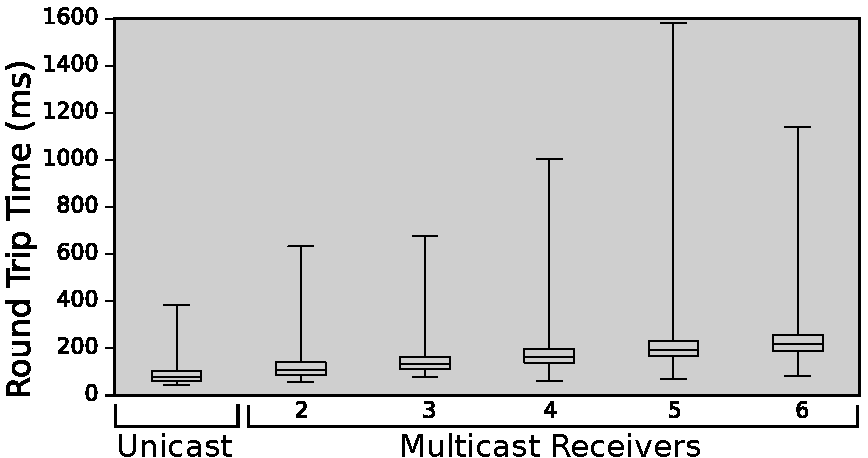
\includegraphics[width = .49\textwidth]{figures/single-hop-group-ps.pdf}
	}

	\subfigure[Publish/Subscribe - Multi-hop] {\label{fig:mhgps}
	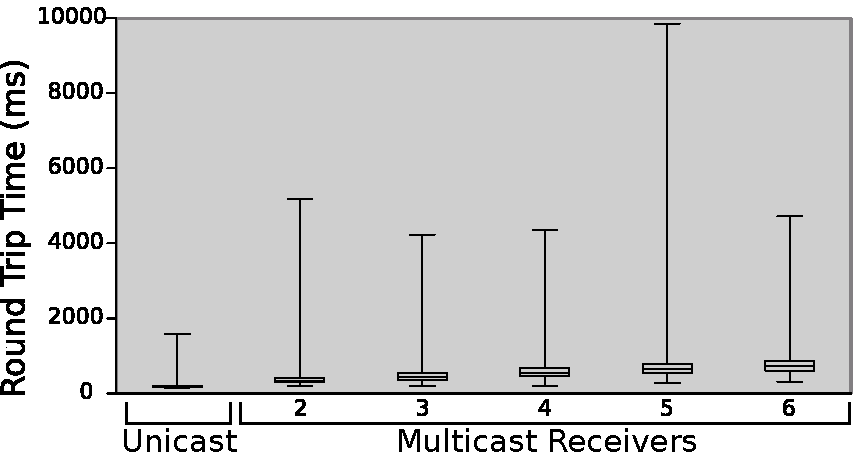
\includegraphics[width = .49\textwidth]{figures/multi-hop-group-ps.pdf}
	}
}
\mbox {
	\subfigure[RPC - Single Hop] {\label{fig:shgrpc}
	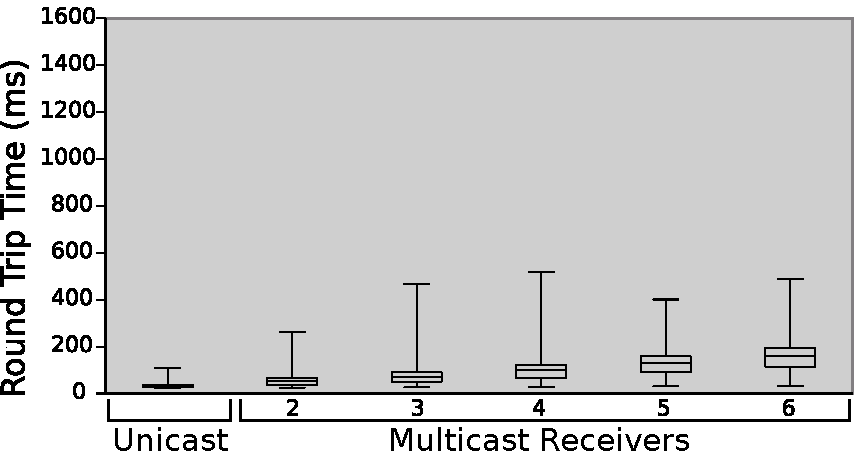
\includegraphics[width = .49\textwidth]{figures/single-hop-group-rpc.pdf}
	}
	
	\subfigure[RPC - Multi-hop] {\label{fig:mhgrpc}
	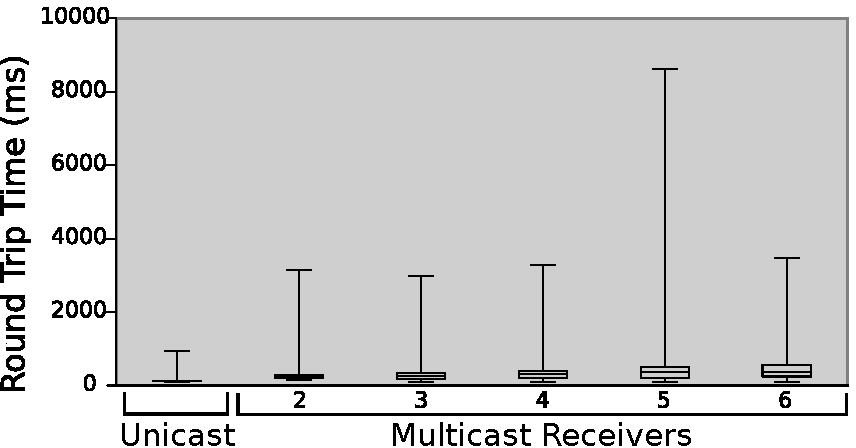
\includegraphics[width = .49\textwidth]{figures/multi-hop-group-rpc.pdf}
	}
}
\mbox {

	\subfigure[Tuple Space - Single Hop] {\label{fig:shgts}
	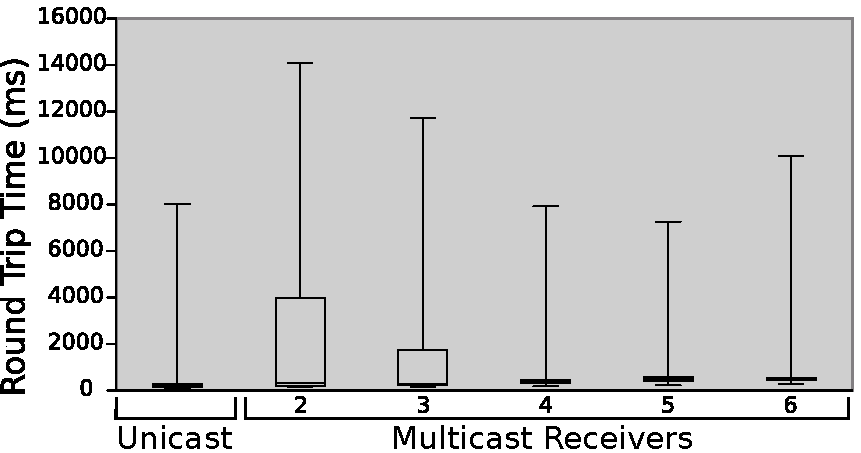
\includegraphics[width = .49\textwidth]{figures/single-hop-group-ts.pdf}
	}

	\subfigure[Tuple Space - Multi-hop] {\label{fig:mhgts}
	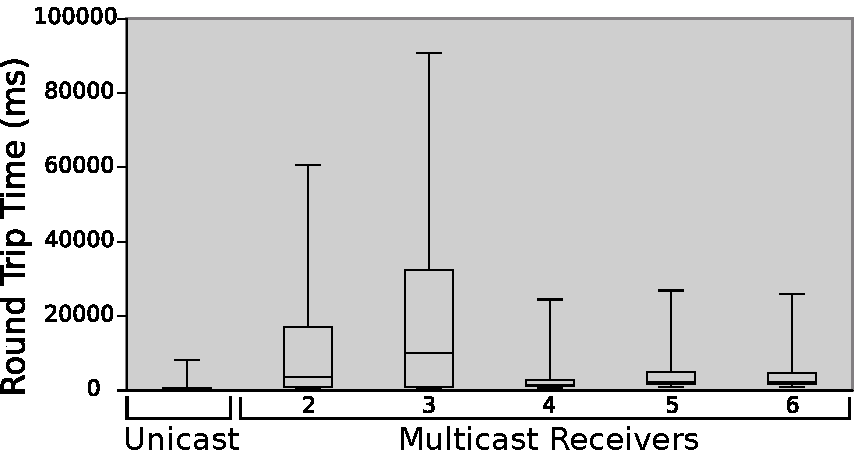
\includegraphics[width = .49\textwidth]{figures/multi-hop-group-ts.pdf}
	}
}
\mbox {
	\subfigure[Publish/Subscribe - Mobile] {\label{fig:mgps}
	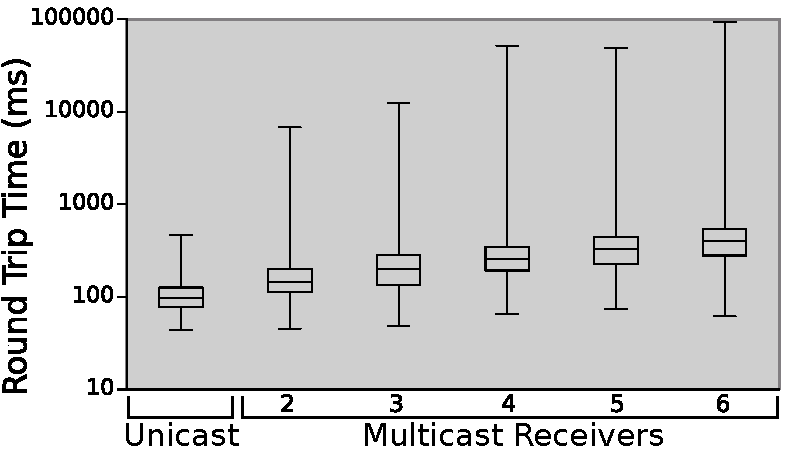
\includegraphics[width = .49\textwidth]{figures/mobile-group-ps.pdf}
	}
	
	\subfigure[RPC - Mobile] {\label{fig:mgrpc}
	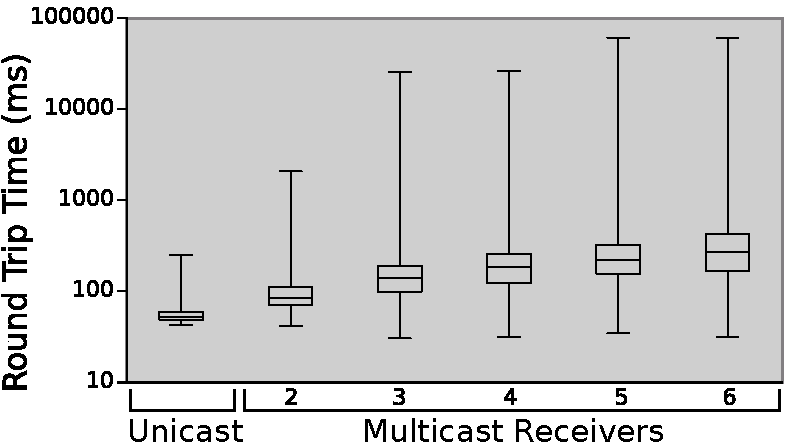
\includegraphics[width = .49\textwidth]{figures/mobile-group-rpc.pdf}
	}
}
	\subfigure[Tuple Space - Mobile] {\label{fig:mgts}
	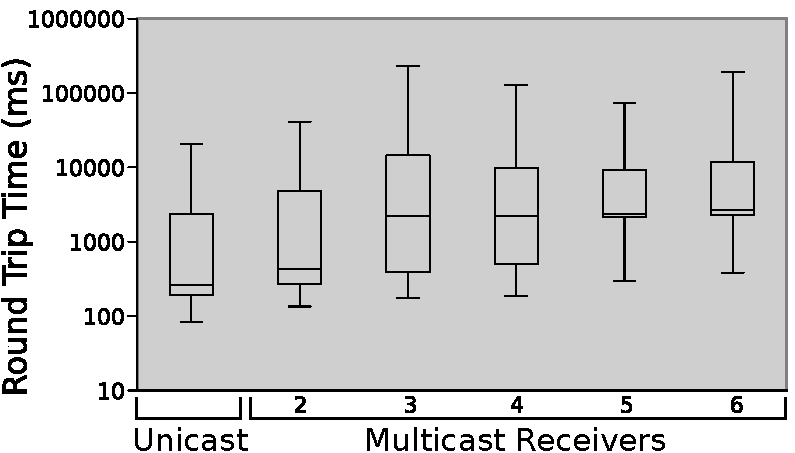
\includegraphics[width = .49\textwidth]{figures/mobile-group-ts.pdf}
	}

\caption{Round Trip Times}
\end{figure}

\subsubsection{Message Delay}\label{sec:group_delay}

We again consider round trip time for each of the paradigms, but this time with an increasing number of receivers. Figures \ref{fig:shgps} - \ref{fig:mgts} show the results for each paradigm and scenario.

For the single hop and multi-hop scenarios, where there is no mobility, the majority of the round trip times are fairly fast. The bottom 75\% of the messages have very similar results, while the top 25\% varies much more. This indicates that an application can expect most messages to be delivered quickly or not at all, but about a quarter of the messages may arrive up to minutes later.

The median delay does increase as receivers are added, especially in the mobile scenario. In the static scenario, the median delay publish/subscribe increased 121\textit{ms} from two receivers to six receivers. RPC increased 147\textit{ms}, and tuple spaces increased 140\textit{ms}. For the mobile scenario, the median times for publish/subscribe increased 255\textit{ms}, RPC increased 237\textit{ms}, and tuple spaces increased by 2035\textit{ms}. The maximum delay values varied much less predictably. For tuple spaces, the static scenarios have unusually long delays with two and three receivers. In the static scenarios, the first three receivers are located in close proximity. One node would dominate the channel for several seconds before relinquishing it. Once again, this shows how influential the wireless channel is on the performance and behavior of applications in MANETs.

The median and maximum tuple space results are much longer than the other two paradigms. The median delay for tuple spaces ranges from twice as much as publish/subscribe in the single hop scenario up to 6 times as high in the mobile scenario. For publish/subscribe and RPC, the majority of delays can only be caused by the network, since they do not attempt to retransmit messages. Tuple spaces, on the other hand, can have very large delays due to the paradigm itself.
%Note that steps 1 and 2 in Figure \ref{fig:tuple-failure} can be reversed: the outgoing tuple can be timestamped before it is even requested by the receiver.
If a receiver is ``behind" it may spend time receiving older tuples before the newest tuple is requested. This causes the round trip times to increase while only improving one-way message delivery.
% While it does improve one-way message delivery, it does not improve the round trip message delivery ratio, due to the reasons discussed in Section \ref{sec:group_reliability}.

\subsection{Shared Whiteboard Application}

When testing the whiteboard application, we considered the metrics which a user might care about at the application level: how reliably and quickly users receive updates.
%This models a classroom or presentation setting where the instructor or presenter is the only one writing on the shared whiteboard, but the contents of the whiteboard are shared out to the class or audience. As in the group communication experiments, in each scenario Node 1 is the sender, with the other nodes marked with triangles as the receivers.
In the results below, a single user is updating the whiteboard and the updates are propagated to 6 receivers. We used traffic traces from  Coccinella\footnotemark to ensure our implementation accurately represented a typical whiteboard application. For these experiments, 250 whiteboard update messages of varying sizes were sent out over a 10 minute period at varying intervals.

\footnotetext{http://thecoccinella.org/}

Furthermore, we tested the whiteboard application under the two different routing protocols we have been using, AODV and DSR. This is not meant to be an exhaustive comparison of the routing protocols themselves, but is intended to show how the choice in routing protocols might affect the performance of the communication models in a nontrivial application.

\begin{figure}
\centering
\mbox {
	\subfigure[DSR] {\label{fig:wbdeliverydsr}
	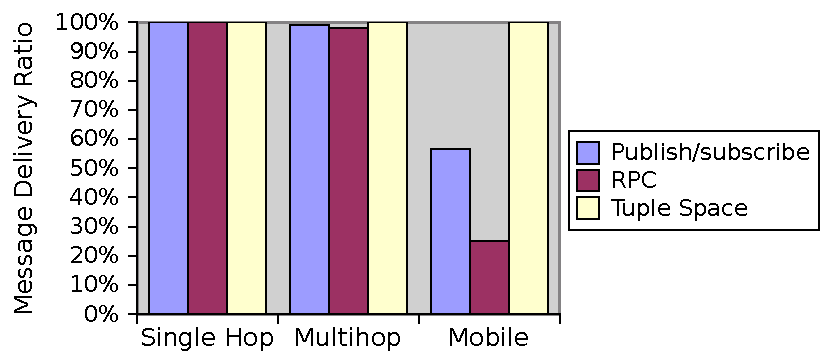
\includegraphics[width = .55\textwidth, clip, trim = 6px 0px 4px 0px]{figures/wb-dsr-delivery.pdf}
	}

	\subfigure[AODV] {\label{fig:wbdeliveryaodv}
	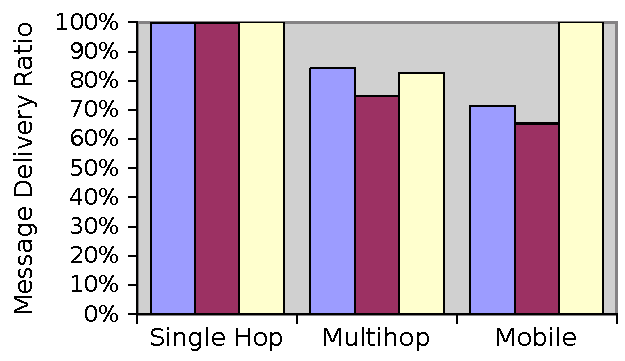
\includegraphics[width = .41\textwidth, clip, trim = 6px 0px 2px 0px]{figures/wb-aodv-delivery.pdf}
	}
}
\caption{Whiteboard Message Delivery}
\end{figure}

\subsubsection{Message Reliability}

Unlike the previous results, these represent one-way communication from the whiteboard user to the receivers. Message reliability determines how accurately the receivers' views reflect the state of the shared whiteboard.

Figures~\ref{fig:wbdeliverydsr} and ~\ref{fig:wbdeliveryaodv} show the percentage of whiteboard messages delivered for DSR and AODV, respectively. As before, the results are nearly 100\% for all paradigms and both protocols in the single hop network. AODV performs poorly on the multi-hop scenario, while DSR achieves nearly 100\% delivery for all paradigms. On the other hand, DSR performs much worse in the mobile scenario, with the delivery ratio for RPC only reaching 25\%.

The reliability of tuple spaces is considerably better in these experiments than in the round trip scenario, with 100\% delivery in all but the AODV multi-hop scenario. The difference between these results and Section \ref{sec:group_reliability} is the lack of a return message. Each receiver is responsible for requesting the whiteboard updates, so the blocking request will be retried until the tuples are received. The only exception is the multi-hop scenario with AODV, in which all three paradigms perform much worse. Since all three paradigms are affected equally, these results must be directly due to the behavior of AODV in this scenario. Investigation of this phenomenon is outside the scope of this paper.

%While the choice of routing protocol can have a significant effect on the paradigm performance, it appears to affect each paradigm in the same manner. In other words, neither routing protocol improves the performance of one paradigm while causing a different paradigm to perform worse.

\begin{figure}
\centering

\mbox {
	\subfigure[DSR] {\label{fig:wbdelaydsr}
	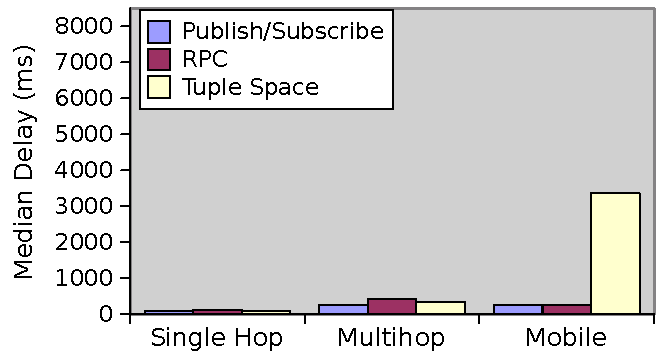
\includegraphics[width = .49\textwidth, clip, trim = 6px 0px 4px 3px]{figures/wb-dsr-delay.pdf}
	}

	\subfigure[AODV] {\label{fig:wbdelayaodv}
	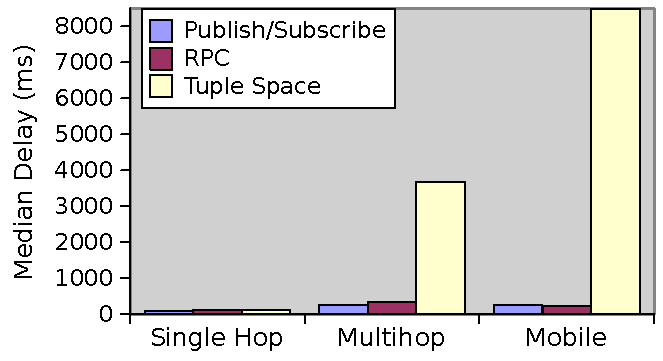
\includegraphics[width = .49\textwidth, clip, trim = 6px 0px 2px 3px]{figures/wb-aodv-delay.pdf}
	}
}
\caption{Whiteboard Message Delay}
\end{figure}


\subsubsection{Message Delay}

Message delay is measured as the time from when a whiteboard update is sent by the application until it is delivered to the receiver's whiteboard. Update delays are very noticeable in a shared whiteboard application, so the delay time should be minimized.

Figure~\ref{fig:wbdelaydsr} shows the results when using DSR and Figure~\ref{fig:wbdelayaodv} shows the AODV results. Not unexpectedly, tuple spaces have the highest median latencies of 8,486\textit{ms} with AODV and 3,357\textit{ms} with DSR. For publish/subscribe and RPC, the median delay remained under 400\textit{ms}.
%As noted previously, there is a direct relationship between reliability and the message delay time. If a message cannot be delivered immediately, the communication paradigm can either drop the message or retry later. Dropping the message decreases reliability, but the median message delay will be low. However, attempting to deliver the message later increases both reliability and message delay.

With DSR, tuple spaces report a nearly 100\% delivery ratio in every scenario, yet the delay times are $<$400\textit{ms} in the static scenarios. In contrast, AODV causes long delays for tuple spaces in both the multi-hop and mobile scenarios. Since tuple spaces will repeatedly attempt to deliver messages, retries are expected to contribute to the majority of the delays. This is supported by the long delay times experienced by tuple spaces with AODV in the multi-hop scenario. However, in the mobile scenario tuple spaces achieve 100\% delivery with AODV and DSR, but the median delay with DSR is less than half as with AODV.

From the mobile reliability results, we can infer that DSR does not maintain viable routes, because the results of publish/subscribe and RPC are poor. However, the delay results suggest DSR is faster than AODV at finding new routes when they become available.

\section{Related Work}

There are many projects using publish/subscribe, RPC, and tuple spaces specifically in MANETs. M2MI (Many-to-Many Invocation)\cite{m2mi} adapts RPC to a MANET context. LIME (Linda in a Mobile Environment)\cite{lime} is a tuple space implementation intended for mobile devices. STEAM (Scalable Timed Events and Mobility)\cite{steam} is an example of an event-based middleware which uses publish/subscribe for communication.

Middleware for MANETs is surveyed in \cite{mwtrends} and \cite{mwsurvey}, but no quantitative results are presented. Projects using different communication paradigms were compared in \cite{mine}. \cite{psvsts} implements tuple spaces in terms of a modified publish/subscribe, but does not provide quantitative results.

\footnotetext{http://www.isi.edu/nsnam/ns/}

\section{Conclusions}

Publish/subscribe, remote procedure calls, and tuple spaces are three communication paradigms which have been applied to MANETs. They have been used as the basis for many projects and applications intended to operate in MANETs. This paper presented a quantitative comparison of these three paradigms in three different network scenarios, with a focus on application level metrics. The results show the relative strengths and weaknesses in each of the three paradigms, as well as how they varied within the same scenario.

Publish/subscribe and RPC provide fast delivery of messages (best times were $<$100\textit{ms}), but provide little message reliability (as low as 25\% delivery ratio for RPC). Tuple spaces, on the other hand, pay a speed penalty (median round-trip times are 2-6 times slower than publish/subscribe), but provide better reliability, since messages will persist until explicitly removed from the tuple space. When used to implement a whiteboard application, tuple spaces achieved a 100\% delivery ratio in all but one scenario.
%However, the pull nature of tuple spaces (see Section \ref{sec:group_reliability}), can undermine group communication reliability.

The wireless channel itself can cause unexpected delays in message delivery. In the single hop scenario, publish/subscribe had a maximum delay of 1.6\textit{s} and tuple spaces had one message require 14\textit{s} to deliver. Introducing multi-hop routes without mobility caused median delay times to double for publish/subscribe and increase by a factor of 10 for tuple spaces. Mobility and multi-hop wireless routes, both defining characteristics of MANETs, strongly influenced the application-level performance and reliability of these paradigms.

%Since these paradigms were not originally intended for MANETs, they do not directly address the challenges of frequent disconnections and mobile nodes. Modifications can and have been made to the basic paradigms in order to handle these shortcomings. 
%For example, introducing a distributed system of brokers can improve message reliability for publish/subscribe, but it also introduces a new level of complexity, since a new mechanism must be introduced for handling the mobility of the brokers themselves.
%Another common approach is to use these paradigms as the core for middleware, which then handles mobility, disconnections, and message delivery.

Our results provide essential quantitative data for deciding which communication model should be used for new projects. While the paradigms presented here are essentially interchangeable in terms of functionality, their performance varies widely according to traffic and wireless conditions. Since we have tested canonical implementations of each paradigm, these results are applicable to basic versions of the paradigms in general and can be used to inform future work in application development for MANETs.

\bibliographystyle{unsrt}
\bibliography{refs}

\end{document}
